\chapter{Concluding remarks}

This thesis has presented the numerical study of Brownian motion in complex environments. Various cases have been considered, from the simple case of free Brownian motion, to rigid confinement and dense suspensions, soft and fluctuating confinement, fluid flow advection on a Brownian solute, and active Brownian motion in quiescent fluids and in fluid flows. 
These various cases were studied using a combination of analytical and numerical methods, with the latter being the main focus and tool. Three publications were produced, and two were presented in their respective chapters. Furthermore, collaborations regarding chapter 2 on hydrodynamic interactions in confined geometries are still ongoing, and a conclusion should be reached in the near future. A similar collaboration involving slip boundary conditions effects on the diffusivity of packed suspensions is also in preparation at the time of writing this manuscript.

\subsection*{Beyond the superimposition of hydrodynamic contributions}

Diffusion is anisotropically and inhomogeneously modifies by confinement. This, in turn, modifies the statistical properties of Brownian displacements~\cite{millan_numerical_2023}. Furthermore, the presence of other colloids in the vicinity of a colloid of interest perturbs the fluid flow and modifies the diffusion of that colloid in a hydrodynamic coupling. In chapter 2, we have seen that the superimposition of hydrodynamic contributions from the confining walls is not sufficient to describe the dynamics of a Brownian particle in a confined geometry. The superimposition of hydrodynamic contributions, namely from Oseen~\cite{Oseen_1927} and Blake~\cite{Blake_1971} approximations, is a common approximation used in the literature~\cite{Dufresne_2000}. However, we have shown that this is not a satisfying theory for any system, and that it leads to significant errors in the prediction of the dynamics of a confined geometry where the colloid is both very close to confinement and to another colloid. The issue is that the superimposition of hydrodynamic contributions does not take into account the coupling between the two walls and the colloid, which is a three-body problem.

By using an image system, it becomes possible to reach higher orders of accuracy. This has been shown experimentally and theoretically already, and we reproduce these results numerically. However, this remains an approximation, and the question of the real dynamics in highly confined regimes remains open. We can reach higher fidelity by using asymptotic corrections to the image system. Still, the full three-body problem cannot be solved analytically, which is another argument for the use of numerical methods with good corrections and high computational efficiency. An experimental investigation is currently being carried out in an effort to strengthen the preliminary results in this chapter, and we are exploring more regimes and other numerical methods for comparison and efficiency purposes. 



\subsection*{Softness can enhance diffusion}
Confinement is not always rigid, and some studies, mostly experimental~\cite{fares_observation_2024} but also theoretical and numerical~\cite{ye_brownian_2025}, have demonstrated various new effects due to the deformability of either the confinement or the colloid itself. In chapter 3, we have seen that the softness of the confining walls can enhance the diffusion of a nearby trapped Brownian particle. Due to the fact that the soft walls can fluctuate, these fluctuations can lead to an effective diffusion coefficient that is larger than the one predicted by the confinement-free case. This has been shown both analytically and numerically. Our model is, however, largely minimal. Other studies based upon our findings should provide more insight on the effect of softness on diffusion, namely in more realistic, three-dimensional geometries with distance-dependent hydrodynamic interactions, or with higher dimensionality. A study involving inertia is also mandated, as our model is in the overdamped limit, and could reveal interesting added-mass effects. 



\subsection*{Microswimmers disperse like Brownian particles}
\begin{wrapfigure}{r}{0.4\textwidth}
    \centering
    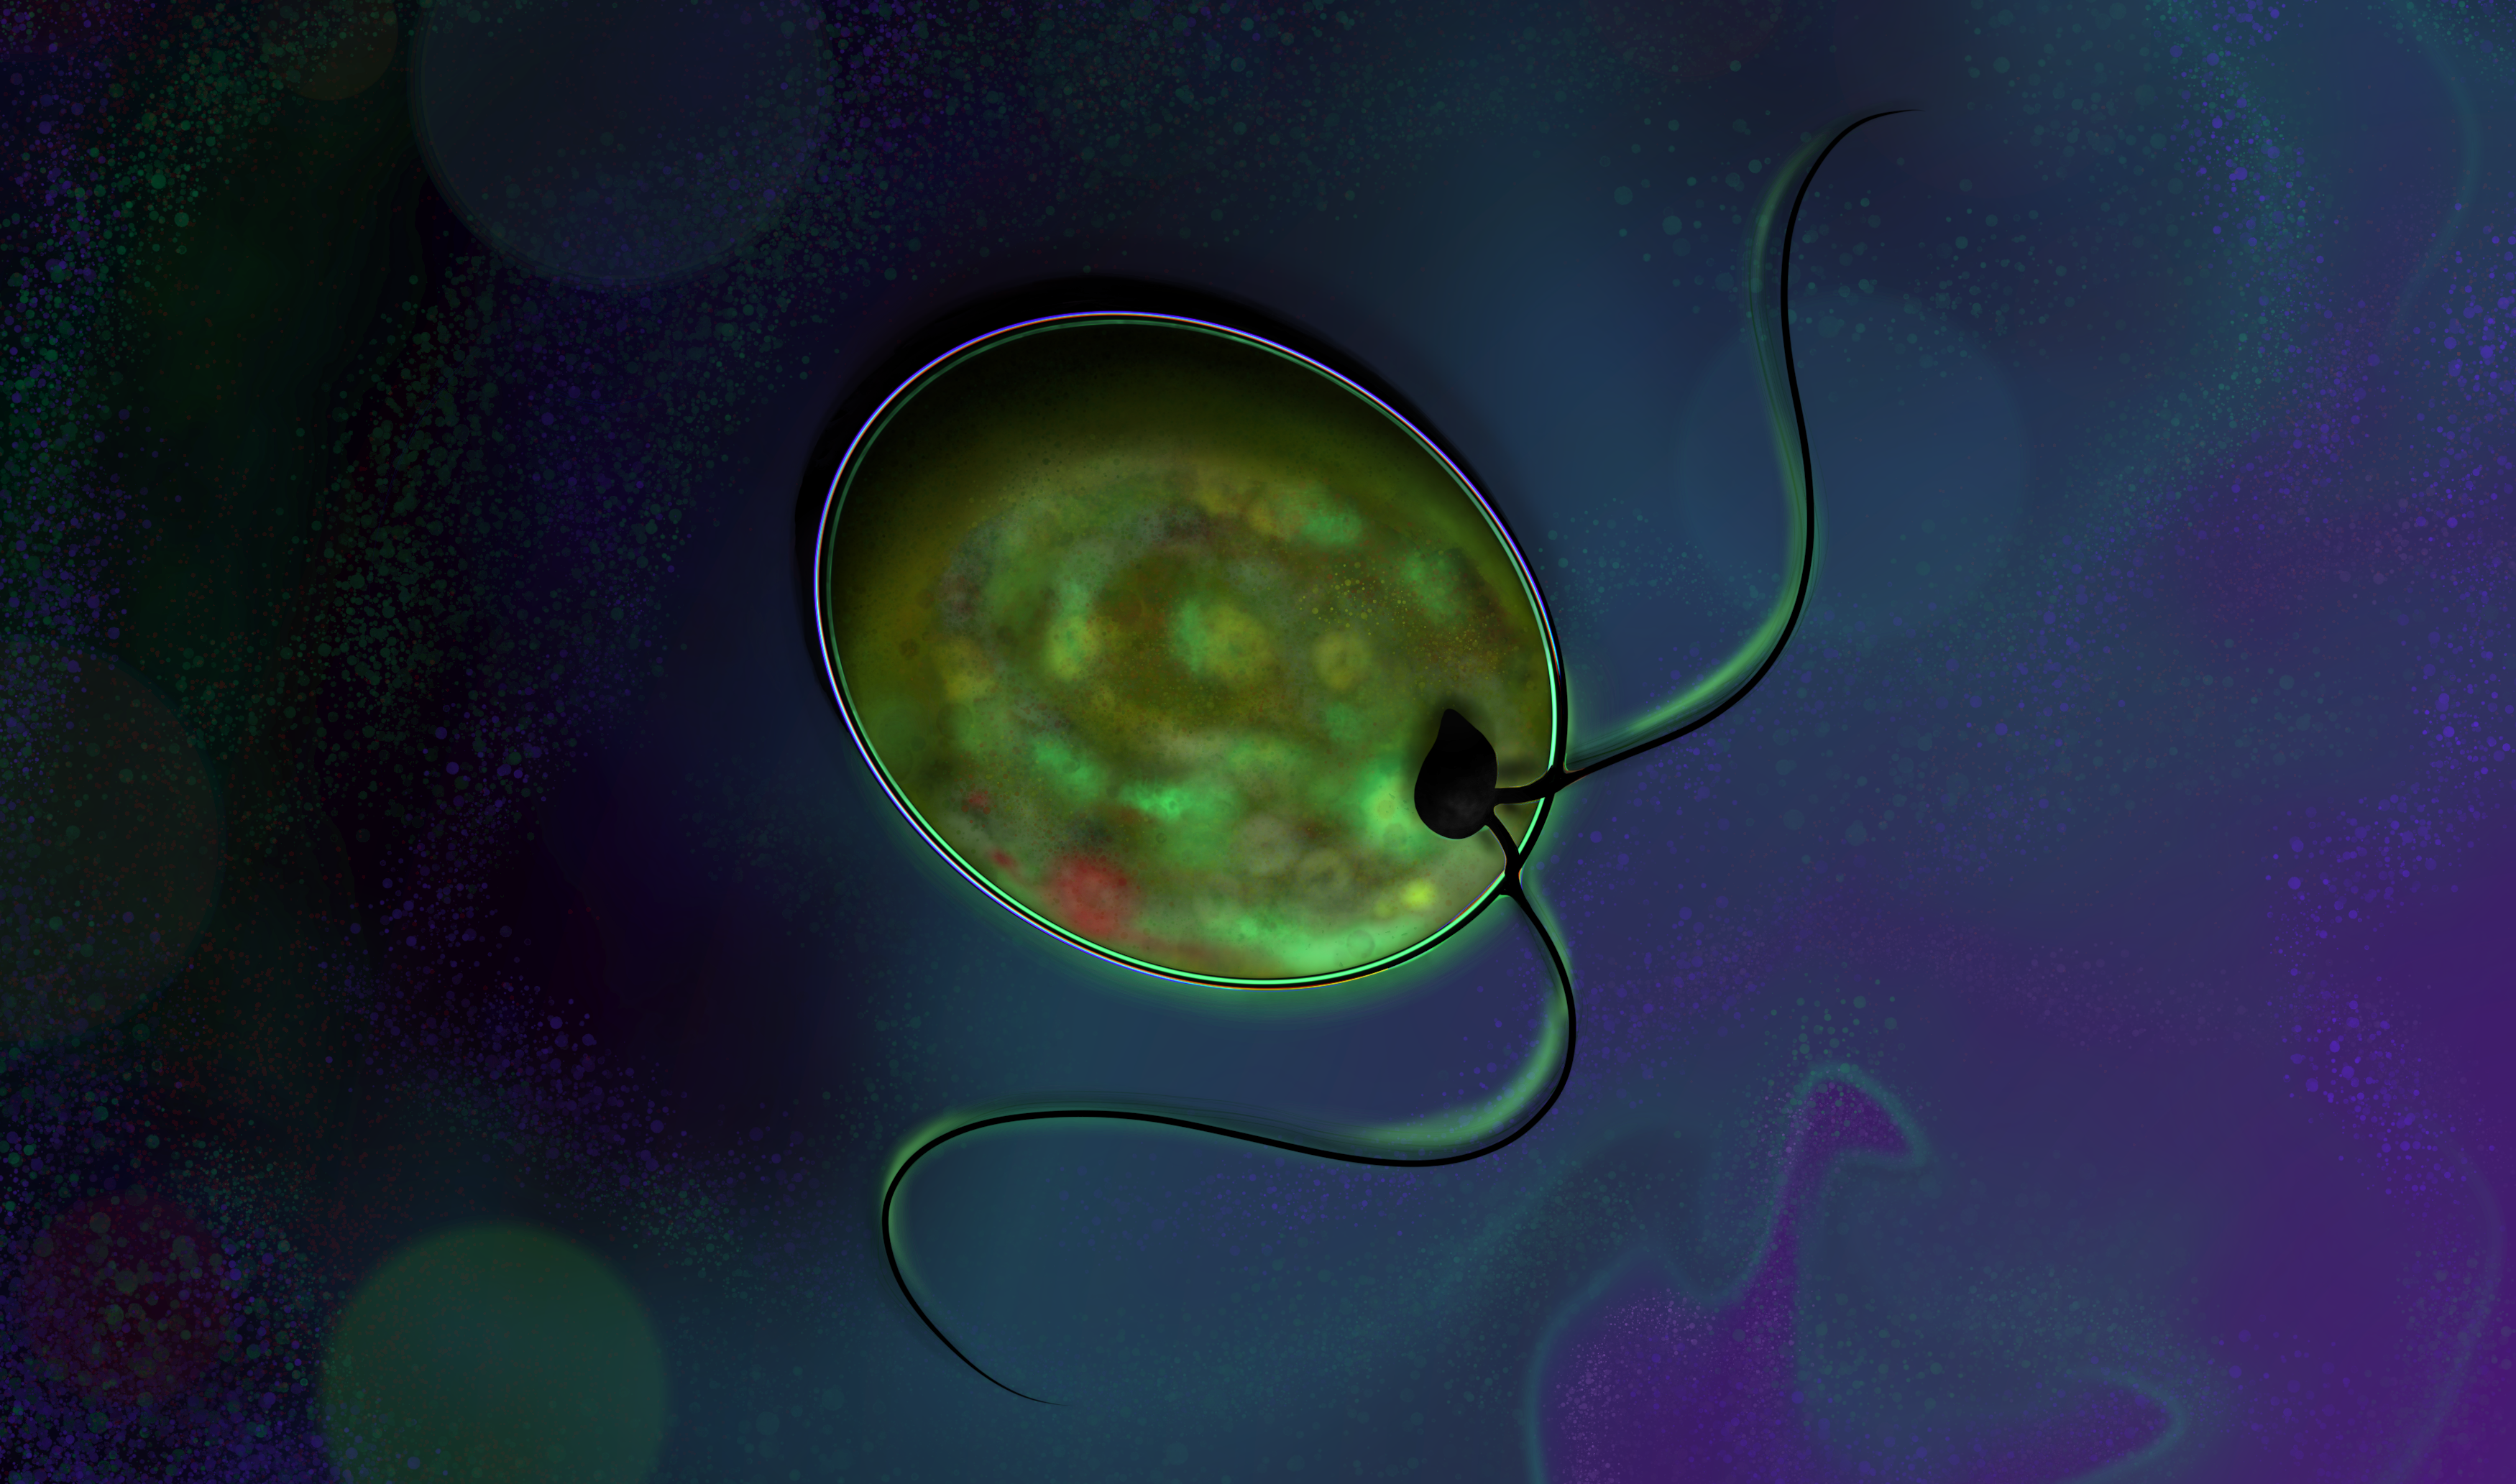
\includegraphics[width=0.40\textwidth]{figures/ccl/CoverPNASLagoin-2k.png}
    \caption[
        Artist's rendition of a \emph{Chlamydomonas reinhardtii} alga swimming. Credits to Elodie Millan.
    ]{
        Artist's rendition of a \emph{Chlamydomonas reinhardtii} alga swimming. Credits to Elodie Millan.
    }
    \label{diedie}
\end{wrapfigure}
Extremely simple mathematical models can suffice to describe the dynamics of a suspension of microswimmers~\cite{marchetti_hydrodynamics_2013,ramaswamy_active_2010,bechinger_active_2016}. In Chapter 4, we describe the behaviour of a plain Brownian solute in advection, but these findings are quickly relevant in chapter 5, where we consider a similar dilute suspension of \emph{Chlamydomonas reinhardtii} (Fig. \ref{diedie}). We find that the dispersion of such an active solution is predicted with the same laws as a passive solute~\cite{taylor_dispersion_1953, taylor_conditions_1954, taylor_turbulent_1954, aris_dispersion_1956}, with the only difference being the effective diffusivity, which results from a higher effective temperature in the case of the microswimmers. Thought not new conceptually, as active Brownian particle models are largely used to describe the behaviours of microswimmers, we still validate numerically what is observed in experiments and predicted by the passive theory. This is extremely encouraging and invites us to explore more complex microswimmer behaviours. Indeed, one may wonder whether this validation stands for the case of a three-dimensional system rather than a quasi-two-dimensional one, where the existence of equilibrium points along the axis of symmetry of a cylindrical channel constitutes a major difference for puller microswimmers. One may also wonder what happens for organisms such as \emph{E. coli}, a canonical example of a pusher microswimmer, where we know already that the far-field flow profile is quite different from that of a puller. 

It is also common for swimmers to move in denser suspensions, with higher and more complex confinement effects from the wall and the presence of other swimmers. In that regard, it would be interesting to work with another model involving finite-size effects, and to fully resolve the fluid numerically and through Particle Image Velocimetry methods experimentally. Furthermore, this case would allow me to couple every bit of knowledge I have accumulated in this PhD, as it would involve the study of hydrodynamic interactions in confined geometries, the effects of softness on diffusion, and the behaviour of microswimmers in a dense suspension. With full control over each of these ingredients, I am certain we could reach a better global understanding of swimmer dynamics in complex environments, and tend to a more general theory of microswimmer dynamics in biological instances.
